%~ \documentclass[letterpaper,times,draft]{sae}
\documentclass[letterpaper,times]{sae}

\usepackage[svgnames]{xcolor}
\definecolor{SAEblue}{RGB}{1,160,233}
%\raggedright

\usepackage[justification=justified, singlelinecheck=false]{caption}  % ,figurename=Fig.,labelfont={it}
\DeclareCaptionFont{eightpt}{\fontsize{8pt}{11pt}\selectfont #1}
\captionsetup{font={eightpt,color=SAEblue}}

\usepackage{lineno}
\usepackage[utf8]{inputenc}

\usepackage{array}% http://ctan.org/pkg/array (also necessary for width calculations (for vert. lines)))
\newcolumntype{L}[1]{>{\raggedright\let\newline\\\arraybackslash\hspace{0pt}}p{#1}}
\newcolumntype{C}[1]{>{\centering\let\newline\\\arraybackslash\hspace{0pt}}p{#1}}
\newcolumntype{R}[1]{>{\raggedleft\let\newline\\\arraybackslash\hspace{0pt}}p{#1}}

\usepackage{graphicx}
\usepackage{multirow}
\usepackage{amsmath}

% Charge le module graphique tikz
\usepackage{tikz}
\usepackage{pgfplots}
\usetikzlibrary{backgrounds}
\usetikzlibrary{shapes,decorations,shadows,arrows,calc}
\usetikzlibrary{decorations.markings}

\newcommand{\ignore}[1]{}
\newcommand{\todo}[1]{\textcolor{red}{TODO: {#1}}}
\newcommand{\todr}[1]{\textcolor{purple}{CAN CUT: {#1}}}
\newcommand{\todm}[1]{\textcolor{green}{MOVE: {#1}}}
\newcommand{\case}[1]{\mbox{\textit{#1}}}
\newcommand{\textss}[1]{\textsuperscript{#1}}
\renewcommand{\deg}{$^\circ$}


\newcommand{\Figref}[1]{Figure \ref{#1}}
\newcommand{\Figrefs}[2]{Figures \ref{#1} and \ref{#2}}
\newcommand{\Figrefsto}[2]{Figures \ref{#1} to \ref{#2}}
\newcommand{\Tabref}[1]{Table \ref{#1}}
\newcommand*{\dt}[1]{%
\accentset{\mbox{\large\bfseries .}}{#1}}
\usepackage{nameref}
\usepackage{booktabs}

% Define "struts" as suggested by Claudio Beccari in
% a piece in TeX and TUG News, Vol. 2, 1993.
\newcommand\Tstrut{\rule{0pt}{4.6ex}}       % "top" strut
\newcommand\Bstrut{\rule[-0.9ex]{0pt}{0pt}} % "bottom" strut
\newcommand{\TBstrut}{\Tstrut\Bstrut} % top&bottom struts

%%% the following hides the section number while keeping their numbering for proper referencing in toc and \ref
\makeatletter
\def\@seccntformat#1{%
  \expandafter\csname c@#1\endcsname\c@section
  }
\makeatother

\usepackage{subfigure}
\usepackage{multimedia}

\DeclareMathOperator{\sign}{sign}
\newcommand{\quotes}[1]{``#1''}


\PaperTitle{An Immersed-Boundary Approach for Multilayer Ice Accretion Simulations}
\usepackage{calc} % to get proper table widths (subtracting colsep and black lines width

\makeatletter 
\renewcommand\@biblabel[1]{#1. } 
\makeatother
\AddAuthor{Karim Zayni}{Department of Mechanical Engineering, Polytechnique Montr\'{e}al, Montr\'{e}al, Canada}
\AddAuthor{Maxime Blanchet}{Department of Mechanical Engineering, Polytechnique Montr\'{e}al, Montr\'{e}al, Canada}
\AddAuthor{Eric Laurendeau}{Department of Mechanical Engineering, Polytechnique Montr\'{e}al, Montr\'{e}al, Canada}
\PaperNumber{2027-XX-XXXX}
\SAECopyright{2027}



\begin{document}
\maketitle

% ============================================================
% ABSTRACT
% ============================================================

\begin{abstract}

This work presents an immersed-boundary framework for aircraft ice-accretion
simulations designed to reduce the dependence of conventional icing workflows
on body-fitted volume meshes. The geometry is represented implicitly using a
signed-distance level-set field and embedded within a non-conformal background
mesh. A ghost-cell immersed-boundary treatment is used for the
Reynolds-averaged Navier--Stokes flow solver, while both Eulerian and
Lagrangian droplet formulations are extended to the immersed-boundary
representation. Ice thermodynamics are evaluated using a Messinger-based
formulation, and the resulting ice geometry is evolved using a continuous
level-set method on a locally adapted mesh. The methodology is assessed using
canonical droplet-impingement benchmarks and rime and glaze ice-accretion
configurations on a NACA~0012 airfoil. Comparisons with body-fitted
simulations demonstrate close agreement in the predicted collection-efficiency
distributions and ice shapes. The results indicate that immersed-boundary
methods provide a promising alternative for reducing the meshing constraints
associated with multilayer aircraft ice-accretion simulations.

\end{abstract}


% ============================================================
% INTRODUCTION
% ============================================================

\section{Introduction}

Aircraft ice accretion is an unsteady multiphysics process involving
aerodynamic flow, supercooled droplet transport, heat transfer, phase change,
and the progressive evolution of the aircraft surface. Numerical icing tools
generally exploit the difference between the characteristic time scales of
these phenomena through a quasi-steady multilayer formulation. The total
exposure time is divided into discrete accretion steps, during which the
aerodynamic flow, droplet impingement, thermodynamic balance, and geometry
evolution are solved sequentially.

Most numerical icing solvers adopt body-fitted computational meshes
\cite{laurendeau2022summary,laurendeau2024summary}. The flow and droplet
solutions are therefore obtained on a mesh conforming to the instantaneous
aircraft geometry. Following each accretion step, the aerodynamic surface is
updated and the surrounding volume mesh must consequently be deformed or
regenerated before the next solution can be performed.

This requirement represents an important limitation for multilayer
simulations. As the ice geometry becomes increasingly complex, repeated mesh
deformation can deteriorate grid quality and eventually result in highly
skewed or entangled elements. Although automated meshing approaches have
progressed significantly \cite{pointwiseHLPW5}, robust generation of
high-quality meshes around complex three-dimensional ice features remains
challenging, particularly for configurations involving highly irregular
structures such as scallops \cite{broeren2013aerodynamic}.

Immersed-boundary methods offer an attractive alternative by embedding the
geometry within a non-conformal background mesh. The computational grid is
therefore no longer required to conform explicitly to the evolving surface.
Instead, the presence of the solid boundary is introduced through
modifications of the governing equations or reconstructed boundary values.
Several immersed-boundary strategies have been investigated for icing,
including penalization and ghost-cell formulations
\cite{arquis1984conditions,lavoieEuler,lavoieDroplets,pabloIcing,capiGC}.
RANS-based immersed-boundary methodologies have also recently been applied
within the AIAA Ice Prediction Workshop
\cite{laurendeau2022summary,laurendeau2024summary,capi2022,capi2025}.

The present work develops an immersed-boundary icing framework within the
in-house \textsc{CHAMPS} solver. The approach combines a RANS
immersed-boundary flow solver with Eulerian and Lagrangian droplet
formulations, surface thermodynamics, and level-set-based geometry evolution.
The objective is to reduce the dependency of multilayer ice-accretion
simulations on body-fitted volume-mesh generation while retaining the
predictive capability required for aerodynamic, impingement, and
thermodynamic calculations.


% ============================================================
% METHODOLOGY
% ============================================================

\section{Immersed-Boundary Ice-Accretion Framework}

The complete numerical procedure is illustrated in
Fig.~\ref{fig:icingFramework}. For each accretion layer, the aerodynamic flow
field is first computed, followed by the droplet-impingement solution. The
resulting collection efficiency is transferred to the thermodynamic model,
which determines the local ice mass accretion rate. The geometry is then
evolved using a continuous level-set method before the procedure is repeated
for the subsequent layer.

\begin{figure}[htb]
    \centering
    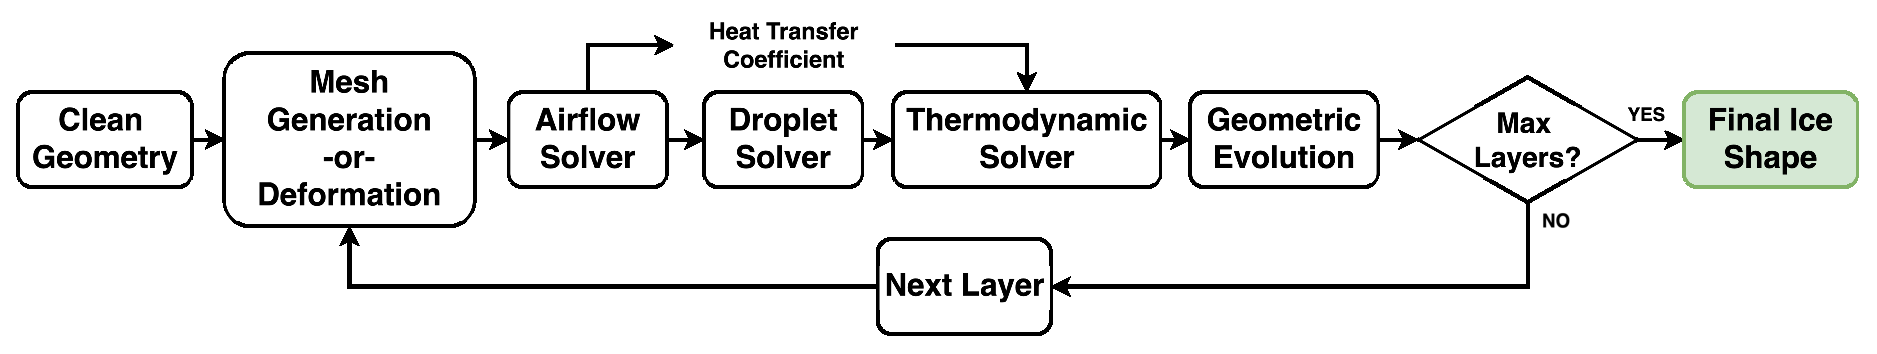
\includegraphics[width=0.88\linewidth]{icingFramework.eps}
    \caption{Multilayer ice-accretion framework combining immersed-boundary
    flow and droplet computations with level-set geometry evolution.}
    \label{fig:icingFramework}
\end{figure}


% ------------------------------------------------------------
% IMMERSED GEOMETRY AND FLOW
% ------------------------------------------------------------

\subsection{Immersed Geometry and Flow Solver}

The immersed geometry is represented using a signed-distance level-set
function $\phi$. The solid region is identified by $\phi<0$, the fluid region
by $\phi>0$, and the immersed surface corresponds to $\phi=0$. The signed
distance is obtained using a ray-casting procedure
\cite{schneider2002geometric}, while the gradient of the level-set field
provides the local surface-normal direction,

\begin{equation}
    \boldsymbol{n}_{\phi}
    =
    \frac{\nabla \phi}{|\nabla \phi|}.
\end{equation}

Unlike a body-fitted formulation, the aerodynamic surface can intersect the
background computational cells arbitrarily. Figure~\ref{fig:meshComparison}
illustrates the difference between the two representations for a circular
cylinder.

\begin{figure}[htb]
\centering
    \subfigure[Body-fitted mesh.]{%
    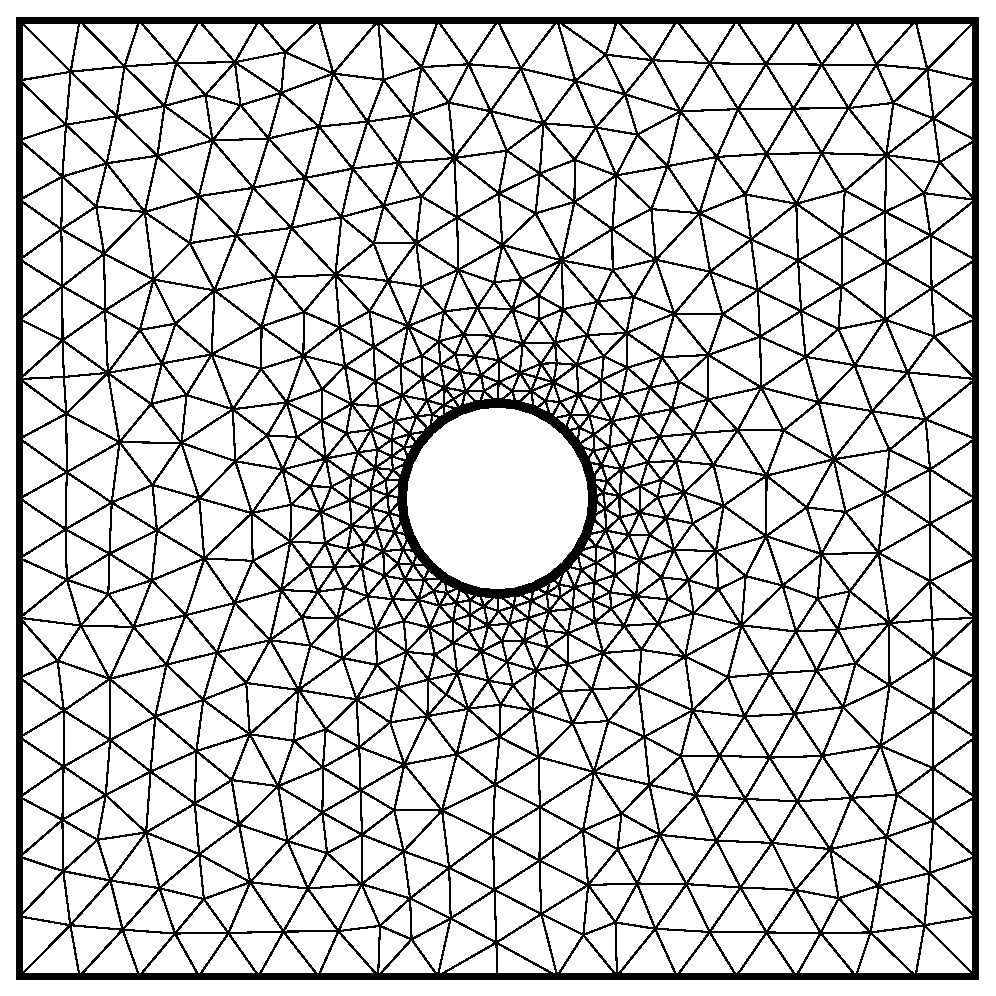
\includegraphics[width=0.42\linewidth]{CYLINDER_BF.eps}}
    \hfill
    \subfigure[Immersed-boundary mesh.]{%
    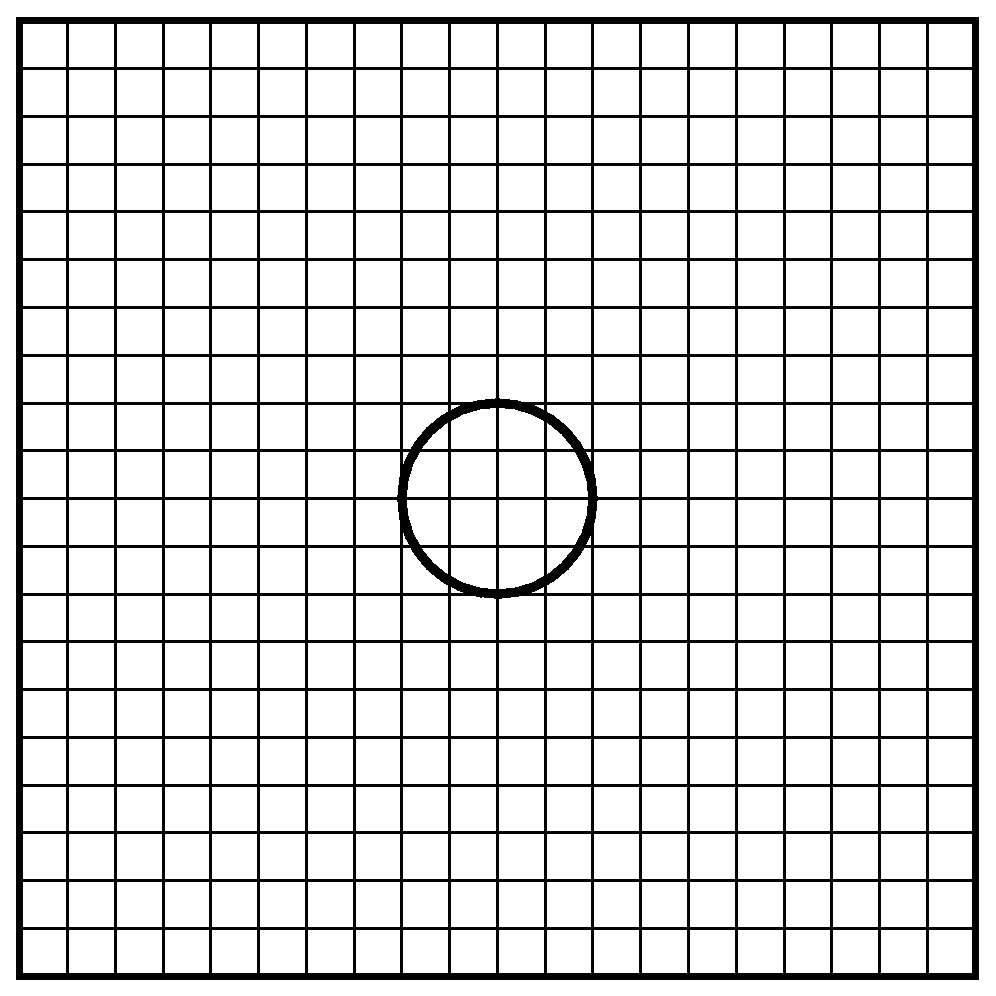
\includegraphics[width=0.42\linewidth]{CYLINDER_IBM.eps}}
    \caption{Body-fitted and immersed-boundary representations of the same
    geometry.}
    \label{fig:meshComparison}
\end{figure}

The aerodynamic solution is obtained from the compressible RANS equations,
with turbulence modeled using the $k$--$\omega$ formulation
\cite{kOmegaMenter}. Wall boundary conditions are imposed using a ghost-cell
methodology based on \cite{CONSTANT2021110240}. Ghost cells located inside
the immersed body are associated with image points in the fluid domain, from
which the required flow quantities are reconstructed. This allows the
boundary condition to be imposed sharply without modifying the connectivity
of the background mesh.


% ------------------------------------------------------------
% DROPLET IMPINGEMENT
% ------------------------------------------------------------

\subsection{Eulerian and Lagrangian Droplet Impingement}

Both Eulerian and Lagrangian descriptions of the dispersed water phase are
considered. Under typical aircraft icing conditions, the droplet phase is
sufficiently dilute for droplet--droplet interactions to be neglected
\cite{guardoneReview}.

In the Eulerian formulation, the droplet conservation equations are solved
directly on the background mesh. The presence of the immersed solid is
introduced through a penalization procedure following the formulation
developed in \cite{lavoieDroplets}. This strategy requires only limited
modification of the original governing equations and allows the same
non-conformal computational mesh to be used for both aerodynamic and droplet
solutions.

The Lagrangian formulation instead computes individual droplet trajectories
through the aerodynamic velocity field. Trajectories are advanced through
the unstructured background mesh following the tracking procedure described
in \cite{rendall2014finite}. Intersection between a droplet trajectory and
the immersed level-set surface identifies an impact event and provides the
information required to reconstruct the local collection efficiency.

The availability of both formulations provides an additional verification
of the immersed-boundary impingement methodology. The Lagrangian formulation
also avoids some of the numerical diffusion associated with Eulerian
transport near sharp impingement limits.

For supercooled large droplets (SLD), additional deformation and splashing
effects are incorporated. Droplet drag is corrected following
\cite{clift2005bubbles}, while the semi-empirical splashing formulation of
\cite{wright2004semi} accounts for the influence of impact angle and kinetic
energy.


% ------------------------------------------------------------
% THERMODYNAMICS AND GEOMETRY EVOLUTION
% ------------------------------------------------------------

\subsection{Thermodynamics and Geometry Evolution}

Surface thermodynamics are evaluated using a Messinger-type formulation
following \cite{Zhu_2014}. The local energy balance determines the fraction
of impinging water that freezes and provides the corresponding ice mass
accretion rate.

The resulting geometry is evolved using a continuous level-set method based
on the formulation of \cite{OSHER198812}. The ice--air interface is
represented by the zero contour of $\phi$ and propagated according to

\begin{equation}
    \frac{\partial \phi}{\partial t}
    + \nabla \cdot \left(\phi\boldsymbol{V}\right)
    - \phi\nabla\cdot\boldsymbol{V}
    =0 ,
\end{equation}

where $\boldsymbol{V}$ represents the local ice-growth velocity. The
magnitude of this velocity is determined from the predicted ice mass
accretion rate and ice density.

Although the aerodynamic and droplet calculations are performed using the
immersed-boundary background mesh, a hybrid strategy is currently adopted
for geometry evolution. The level-set equation is solved on a locally
adapted unstructured mesh refined around the ice-growth region, as shown in
Fig.~\ref{fig:adaptedMesh}.

\begin{figure}[htb]
    \centering
    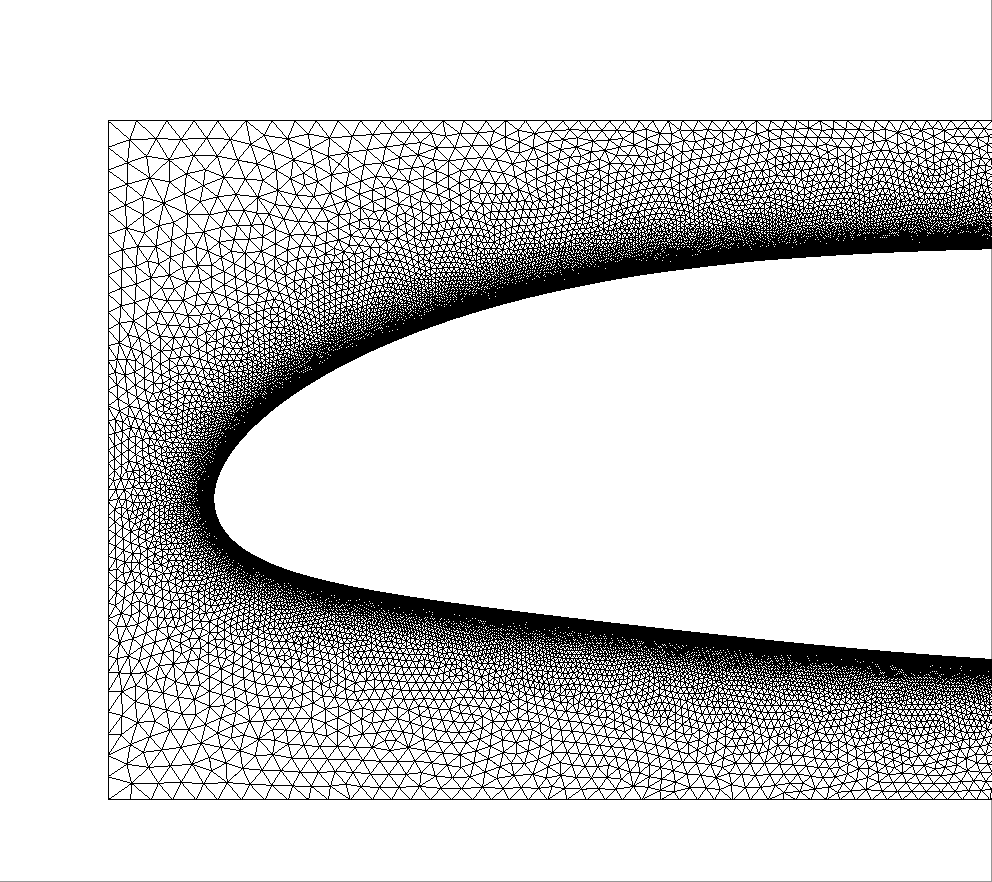
\includegraphics[width=0.52\linewidth]{MESH_ADAPTATION.png}
    \caption{Locally adapted unstructured mesh used for level-set geometry
    evolution around the iced surface.}
    \label{fig:adaptedMesh}
\end{figure}

A semi-implicit Rosenbrock--Wanner integration scheme is employed to reduce
the restrictive time-step requirements associated with explicit level-set
propagation. Following each accretion step, the zero level set is extracted
using the \textsc{MMG} remeshing library \cite{DAPOGNY2014358}, producing
the updated ice surface for the following layer.


% ============================================================
% PRELIMINARY RESULTS
% ============================================================

\section{Preliminary Results}

The immersed-boundary framework is assessed using canonical droplet
impingement cases followed by complete rime and glaze ice-accretion
simulations. A circular cylinder is first considered because an analytical
collection-efficiency solution is available for verification
\cite{lavoieDroplets}. Both the Eulerian and Lagrangian immersed-boundary
formulations recover the expected collection-efficiency distribution and
show close agreement with their corresponding body-fitted solutions.

The methodology is further assessed using the NACA~23012 SLD impingement
benchmark of \cite{papadakism2004water}. Figure~\ref{fig:sld} compares the
predicted collection-efficiency distributions obtained with the Eulerian
and Lagrangian formulations. Inclusion of SLD deformation and splashing
effects improves agreement with the experimental measurements. Both
immersed-boundary formulations reproduce the overall impingement behavior,
although the Eulerian solution exhibits slightly greater numerical smearing
near sharp impingement limits, consistent with previous observations for
Eulerian immersed droplet formulations \cite{lavoieDroplets}.

\begin{figure}[htb]
\centering
    \subfigure[Eulerian formulation.]{%
    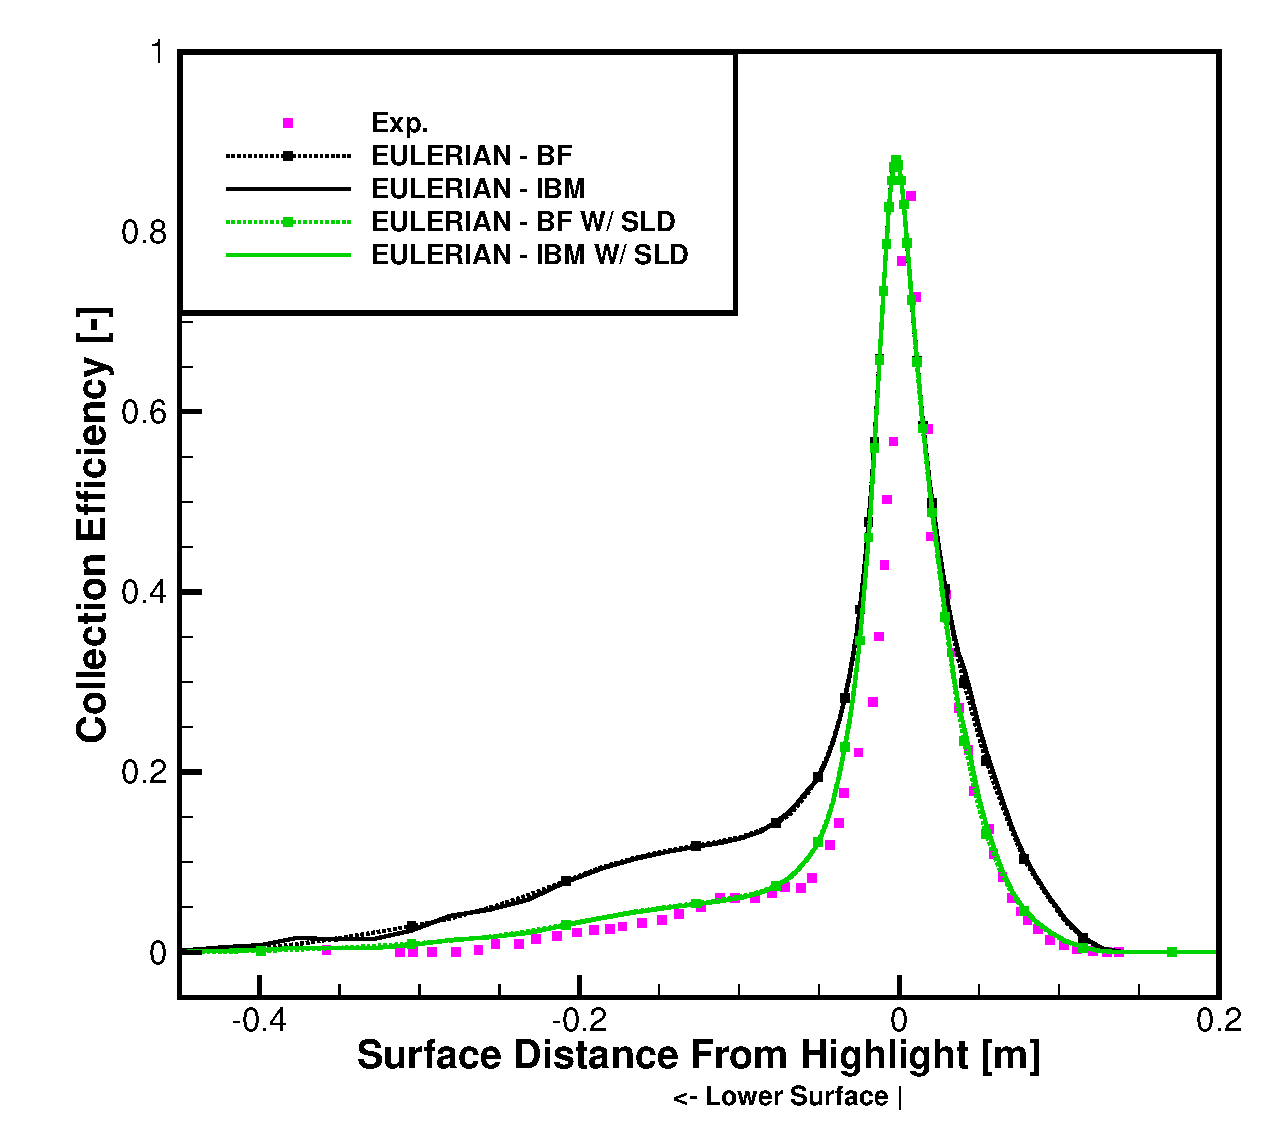
\includegraphics[width=0.48\linewidth]{CASE_SLD_EULERIAN_BETA.eps}}
    \hfill
    \subfigure[Lagrangian formulation.]{%
    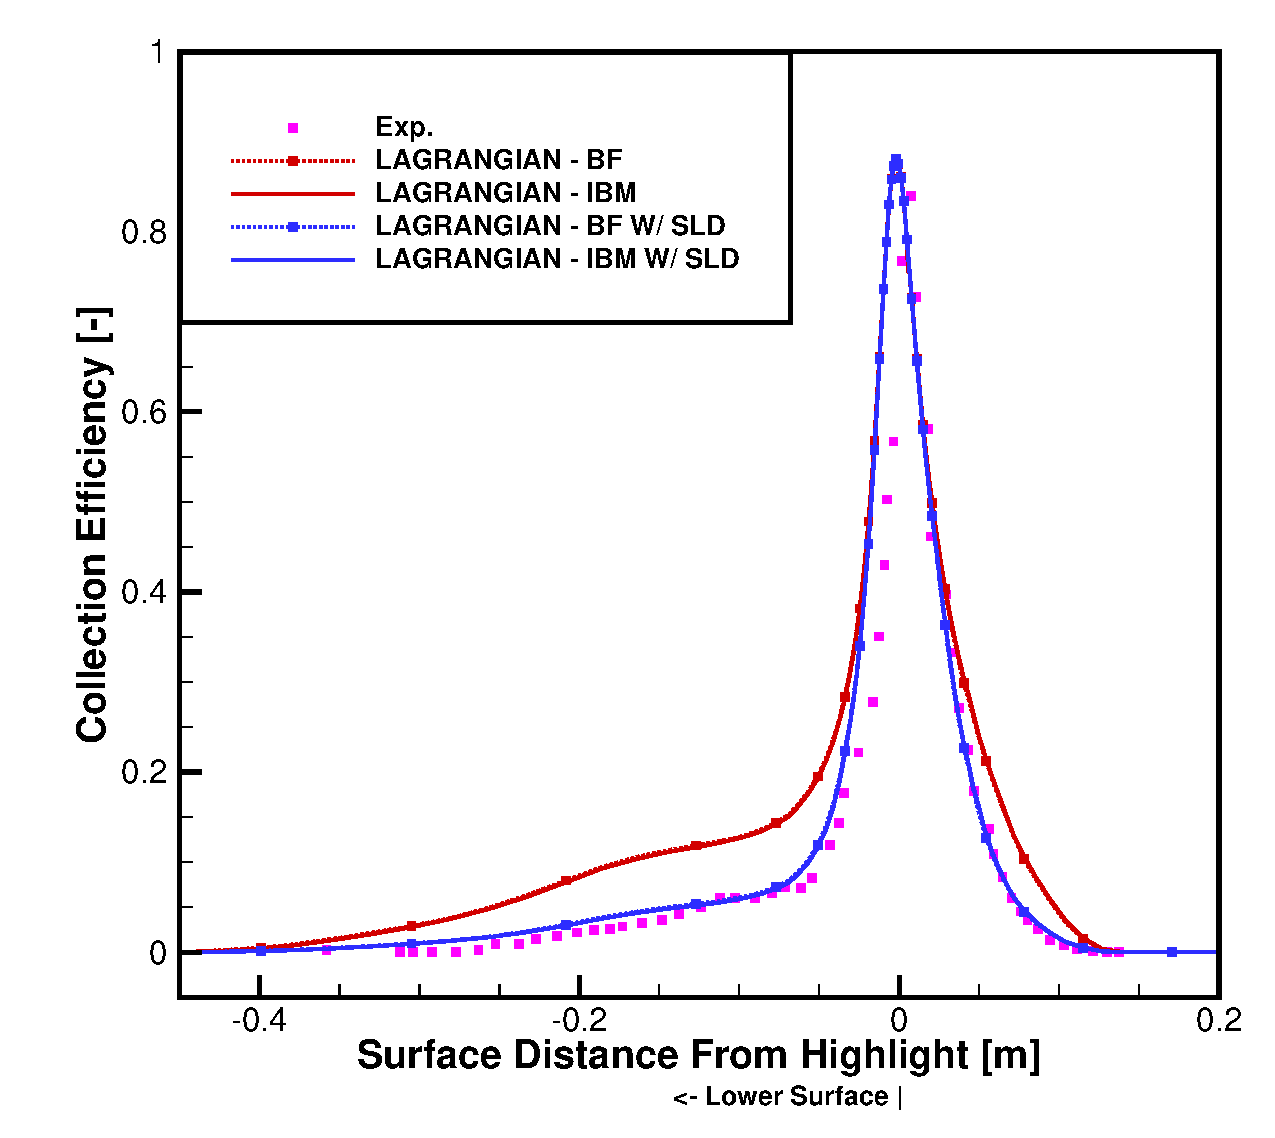
\includegraphics[width=0.48\linewidth]{CASE_SLD_LAGRANGIAN_BETA.eps}}
    \caption{Collection-efficiency distributions for the NACA~23012 SLD
    impingement benchmark of \cite{papadakism2004water}.}
    \label{fig:sld}
\end{figure}

Complete ice-accretion simulations are subsequently performed for rime and
glaze conditions on a NACA~0012 airfoil using the wind-tunnel experiments
of \cite{trontin}. For the rime condition, where the ice geometry is
predominantly controlled by the impingement distribution, the body-fitted
and immersed-boundary predictions are nearly identical. Increasing the
number of accretion layers also improves agreement with the experimental
profile.

The glaze condition provides a more demanding assessment because the
resulting horn geometry depends strongly on the local thermodynamic balance
and convective heat transfer. Figure~\ref{fig:glaze} compares body-fitted
and immersed-boundary predictions after one and five accretion layers.
Both approaches reproduce the principal experimental features, including
the formation of the upper and lower horns. The single-layer predictions
remain close, whereas differences become more visible after five layers.
These deviations are primarily associated with differences in the near-wall
heat-transfer prediction, which accumulate as the geometry evolves.

\begin{figure}[htb]
\centering
    \subfigure[Single layer.]{%
    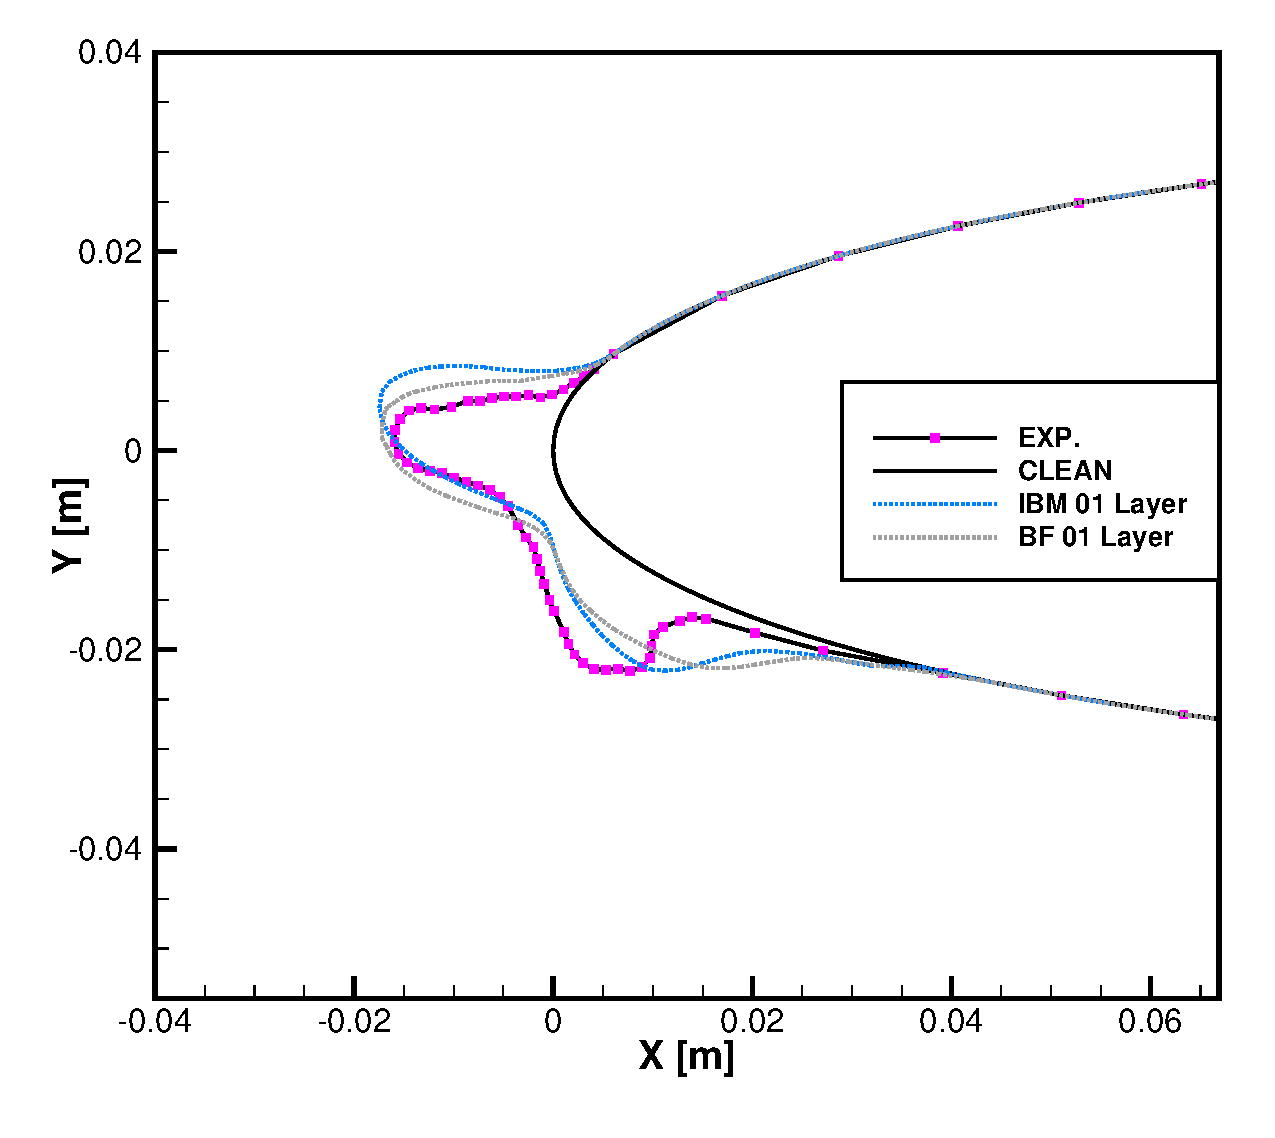
\includegraphics[width=0.48\linewidth]
    {CASE_04_ICE_SHAPE_01_LAYER.eps}}
    \hfill
    \subfigure[Five layers.]{%
    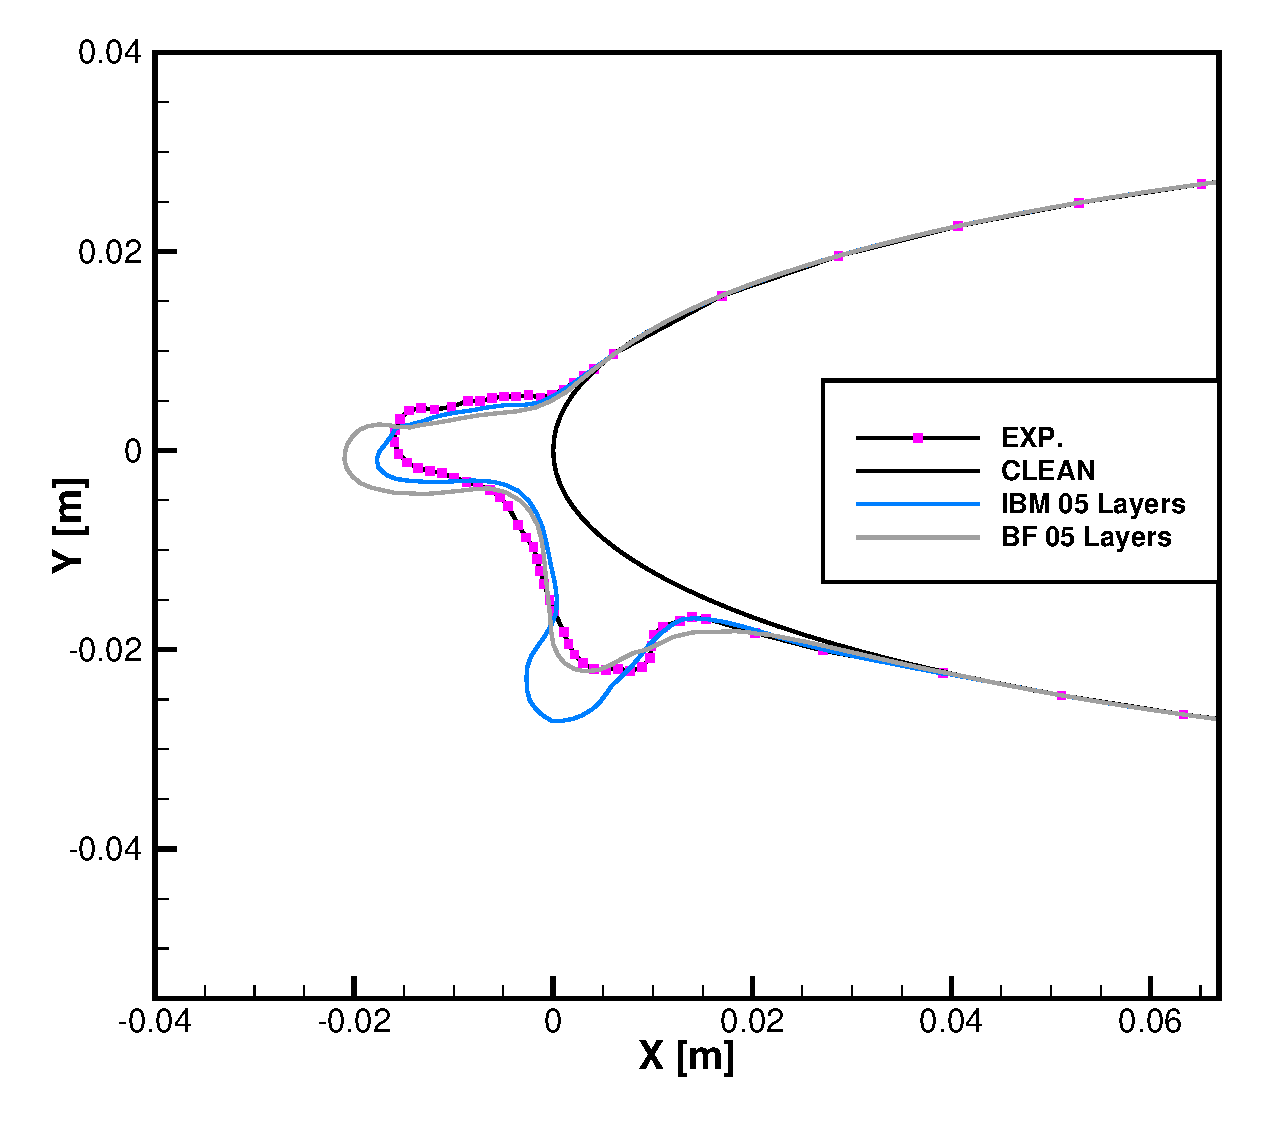
\includegraphics[width=0.48\linewidth]
    {CASE_04_ICE_SHAPE_05_LAYER.eps}}
    \caption{Body-fitted and immersed-boundary ice-shape predictions for
    the NACA~0012 glaze-ice configuration of \cite{trontin}.}
    \label{fig:glaze}
\end{figure}


% ============================================================
% CONCLUSION
% ============================================================

\section{Conclusion and Future Work}

An immersed-boundary framework for multilayer aircraft ice accretion has
been developed within \textsc{CHAMPS}. The methodology combines a RANS
ghost-cell immersed-boundary flow solver, Eulerian and Lagrangian droplet
transport formulations, a Messinger-based thermodynamic model, and
level-set-based geometry evolution. The approach reduces the dependence of
the aerodynamic and droplet calculations on body-fitted volume meshes while
retaining a sharp representation of the immersed surface.

Verification using a canonical cylinder demonstrates that both Eulerian and
Lagrangian immersed-boundary droplet formulations recover the expected
collection-efficiency distribution. Application to the NACA~23012 SLD
benchmark further demonstrates good agreement with experimental impingement
measurements, while the Lagrangian formulation provides a sharper
representation of the impingement limits. Complete rime and glaze
ice-accretion simulations on a NACA~0012 airfoil show that the
immersed-boundary approach produces ice shapes comparable to those obtained
using the body-fitted formulation and captures the principal experimental
features.

The results also identify the aerodynamic and thermal wall treatment as an
important area for further development. While differences between
body-fitted and immersed-boundary solutions remain limited for rime
conditions, small variations in convective heat transfer can accumulate over
successive layers under glaze conditions and influence the final horn
geometry.

Future work will therefore focus on improving the immersed-boundary
near-wall treatment for aerodynamic and thermal predictions and on extending
the methodology to fully three-dimensional ice-accretion configurations.
The longer-term objective is to perform the complete multilayer icing
workflow on non-conformal meshes, further reducing the need for repeated
body-fitted mesh generation as increasingly complex three-dimensional ice
features develop.


% ============================================================
% REFERENCES
% ============================================================
\bibliographystyle{ieeetr} % closest to SAE
\bibliography{references}

\section{Contact Information}
Mohamad Karim Zayni\newline
mohamad-karim.zayni@polymtl.ca

% ============================================================
% ACKNOWLEDGEMENTS
% ============================================================

\section{Acknowledgements}

This work was supported in part by the Canada Research Chairs Program,
the Natural Sciences and Engineering Research Council of Canada (NSERC),
and the Digital Research Alliance of Canada.


% ============================================================
% DEFINITIONS, ACRONYMS, ABBREVIATIONS
% ============================================================

\section{Definitions, Acronyms, Abbreviations}

\begin{table}[h]
\centering
\begin{tabular}{L{0.12\textwidth} L{0.35\textwidth}}
\textbf{CFD}  & Computational Fluid Dynamics \\
\textbf{IBM}  & Immersed-Boundary Method \\
\textbf{RANS} & Reynolds-Averaged Navier--Stokes \\
\textbf{SLD}  & Supercooled Large Droplets \\
\end{tabular}
\end{table}

\textbf{General symbols}

\begin{table}[h]
\centering
\begin{tabular}{L{0.08\textwidth} L{0.29\textwidth} L{0.08\textwidth}}
$\boldsymbol{n}_{\phi}$ & Level-set interface normal & $[-]$ \\
$t$                      & Time                       & $[\mathrm{s}]$ \\
$\boldsymbol{V}$         & Ice-growth velocity        & $[\mathrm{m/s}]$ \\
\end{tabular}
\end{table}

\textbf{Greek symbols}

\begin{table}[h]
\centering
\begin{tabular}{L{0.08\textwidth} L{0.29\textwidth} L{0.08\textwidth}}
$\phi$ & Level-set signed-distance function & $[\mathrm{m}]$ \\
\end{tabular}
\end{table}


\end{document}
